\chapter{Methods and Implementations}

\section{DeepSIM}
\label{sec:DeepSIM}

\subsection{DeepSIM Optical Set-up}
\label{subsec:DeepSIM_optical}

\subsubsection{Optical Alignment}
\label{subsubsec:alignment}

\subsection{Control Software}
\label{subsec:control_software}

\subsubsection{Microscope}
\label{subsubsec:microscope}

\subsubsection{Cockpit}
\label{subsubsec:cockpit}

\section{Introduction}

%% The Introduction should provide context as to why the software tool
%% was developed and what need it addresses.  It is good scholarly
%% practice to mention previously developed tools that address similar
%% needs, and why the current tool is needed.

Many of the recent innovations in biological imaging have revolved around the quest for greater resolving power, ultimately culminating in the advent of super-resolution microscopy techniques. However, there is commonly a difference between the theoretical resolution advertised by any microscopy technique or setup and the practical resolution obtained in biological imaging. This is particularly true for live, thick samples, which are often particularly interesting to biological researchers for their ability to show dynamic biological processes \textit{in situ}. The performance of a given microscope system, how close the theoretical and practical resolutions are to one another, is largely dependent on the optical aberrations present, most of which arise from the heterogeneity of the biological sample itself.\cite{schwertner2004characterizing,schwertner2004measurement} These aberrations compromise image quality by decreasing contrast and resolution by distorting the optical wavefront.\cite{booth2007adaptive,wyant1992basic} Implementing adaptive optics (AO) in microscopy has already been shown to be highly effective at removing these aberrations and yielding significantly improvements to image quality.\cite{booth2014adaptive,girkin2009adaptive} It is therefore not an unreasonable assertion that the widespread use of AO in microscopy would be a significant boon to biological research.

Unfortunately, whilst there have been multiple 'proof-of-principle' AO microscopy setups have been demonstrated, a widespread use of AO has yet to be adopted. This is due, in large part, to the complicated nature of measuring the wavefront deformations (and therefore the aberrations) present in a sample. While direct wavefront measurements do exits, they carry additional complications and are only applicable in certain samples.\cite{wang2014rapid,wang2015direct} Therefore indirect wavefront sensing is generally preferred.\cite{rodriguez2018adaptive} However, most 'proof-of-principle' AO microscopy setups implement a single method of correction that is particularly suited to the specific imaging modality and/or sample being used. So far, a robust, easy-to-use implementation which incorporates multiple AO methods for multiple sample types/imaging modalities has yet to be presented.\cite{ji2017adaptive}

Microscope-AOtools aims to provide such a generalised solution. It utilises Python Microscope, an open-source hardware control software, to provide control over the physical hardware necessary for adaptive optics implementations. It incorporates methods for calibrating a deformable mirror (DM), evaluating the success of the calibration in recreating aberrations and performing both direct wavefront sensing and sensorless adaptive optics corrections. The methods for sensorless adaptive optics correction can utilise a number from a suite of image quality metrics which can be easily extended to include additional sample or imaging method-specific metrics.

\section{Set-up Methods}

\subsection{Calibration}

For aberration correction, one could attempt to measure the overall aberration of the optical wavefront and apply the opposite shape to the DM. For direct wavefront sensing, this would appear as simple as measuring the phase distortion and shaping the DM to cancel this distortion. However, for continuous membrane DMs (which the majority of commercially available DMs are) the response of mirror shape to the actuators which control the mirror shape is generally non-linear, due to the membrane's mechanical elasticity, electrostatic forces and the coupling between actuators.\cite{Zhu:99} For indirect wavefront sensing this presents an even greater problem since any minimisation of the wavefront aberration would involve \textit{N} degrees of freedom, where \textit{N} is the number of actuators. Assuming that the overall mirror shape is the linear superposition of all the individual actuator deflections, we can define the overall mirror shape, $S(x,y)$ as:

\begin{equation}\label{eq:surface_shape}
\Delta S(x,y) = \sum_{l=1}^{N} d_{l}\phi_{l}(x,y)
\end{equation}

Where $\Delta S(x,y)$ is the change in the DM shape from its original position, $d_l$ is the $l$-th actuator control signal (an arbitrary value related to applied voltage which determines the position the $l$-th actuator in its overall movement range)	and $\phi_{l}(x,y)$ is the $l$-th influence function. We can change this orthogonal set of basis functions for a different sensible basis set. An obvious alternative basis set is the Zernike polynomials since the wavefront distortion can be approximated by the linear addition of Zernike polynomials.\cite{von1934beugungstheorie,noll1976zernike} Describing $\phi_{l}(x,y)$ in terms of Zernike polynomials we obtain:

\begin{equation}\label{eq:influence_to_zernike}
\phi_{l}(x,y) = \sum_{k=1}^{M} b_{k,l}z_{k}(x,y)
\end{equation}

Where $b_{k,l}$ is the coefficient corresponding to the $k$-th Zernike polynomial due to the $d_l$. This leads to:

\begin{equation}\label{eq:zernike_sub}
\begin{split}
\Delta S(x,y) & = \sum_{l=1}^{N} d_{l}\left[\sum_{k=1}^{M} b_{k,l}z_{k}(x,y)\right] \\
& =\sum_{k=1}^{M} \left(\sum_{l=1}^{N} d_{l} b_{k,l}\right) z_{k}(x,y) \\
& =\sum_{k=1}^{M} a_{k} z_{k}(x,y)
\end{split}
\end{equation}

Where the new Zernike coefficients, $a_{k}$, is defined as:

\begin{equation}\label{eq:new_z_coef}
a_{k} = \sum_{l=1}^{N} b_{k,l} d_{l} \text{~for~} k=1,2,...,M
\end{equation}

Converting this to a matrix form yields:

\begin{equation}\label{eq:CM_derivation}
\begin{split}
\bar{a} &= \boldsymbol{B} \bar{d}\\
\Rightarrow \bar{d} &= \boldsymbol{C} \bar{a}
\end{split}
\end{equation}

Where $\bar{d}$ is a length $N$ vector of the actuator control signals, $\bar{a}$ is the length $M$ vector of the Zernike polynomial amplitudes and $\boldsymbol{B}$ is the $M \times N$ matrix representing the response characteristics of the DM. However, we actually want its inverse, $\boldsymbol{B}^{-1} =\boldsymbol{C}$, otherwise called the control matrix in order to convert from Zernike polynomial amplitudes to actuator control signals.

Microscope-AOtools implements an automated calibration routine to obtain $\boldsymbol{C}$. Each actuator is moved through a number, $p$, of set positions and a wavefront is extracted. Then $M$ Zernike modes, modelled with a Python package, are then fitted to the wavefront.\cite{townson2019aotools} A row vector $\boldsymbol{z}$ is obtained:

\begin{equation}\label{eq:zernike_amp}
\boldsymbol{z} = 
\begin{bmatrix}
z_{1} & z_{2} & \cdots & z_{m} 
\end{bmatrix}
\end{equation}

Where the $k$-th element is the amplitude of the $k$-th Zernike mode. By collecting the row vectors of each position for each $l$-th actuator we can obtain:

\begin{equation}\label{eq:zernike_amp_actuator}
A_l = 
\begin{bmatrix}
\boldsymbol{z_{1}}\\
\boldsymbol{z_{2}}\\
\vdots\\
\boldsymbol{z_{p}} 
\end{bmatrix}
=
\begin{bmatrix}
z_{1,1} & z_{1,2} & \cdots & z_{1,m} \\
z_{2,1} & z_{2,2} & \cdots & z_{2,m} \\
\vdots  & \vdots  & \ddots & \vdots  \\
z_{p,1} & z_{p,2} & \cdots & z_{p,m} 
\end{bmatrix}
\end{equation}

Fitting linear regression to each column, $\begin{bmatrix} z_{1,i} & z_{2,i} & \cdots & z_{p,i} \end{bmatrix}^T$, yields the response characteristics between the $l$-th actuator's position and the $k$-th Zernike mode, $b_{k,l}$. In this way, we construct $\boldsymbol{B}$ and then calculate $\boldsymbol{C}$. Figure~\ref{fig:Ith_actuator_calibration_workflow} shows a flowchart representing this process for the $l$-th actuator as implemented in Microscope-AOtools. This is process is repeated for all $N$ actuators.

\begin{figure}[h]
	\centering
	\includegraphics[width=0.4\textwidth, scale=0.5]{./images/Ith_actuator_calibration_workflow.jpg}
	\caption{Flowchart depicting the the process for calibrating the $l$-th actuator of the deformable mirror. The influence functions returned are $b_{k,l}$ described in Equation~\ref{eq:influence_to_zernike}. This process is performed for each $N$ actuators and used to obtain $\boldsymbol{C}$ described in Equation~\ref{eq:CM_derivation}.}
	\label{fig:Ith_actuator_calibration_workflow}
\end{figure}

In general, $\boldsymbol{B}$ is singular and therefore has no true inverse and so we must use a pseudo-inverse, calculated using single value decomposition (SVD). However, some values of $\boldsymbol{B}$ may be small since the physical position of certain actuators will mean they have limited influence on creating certain Zernike modes. A control matrix calculated without thresholding out these small values will quickly lead to a saturation of the DM actuators (i.e. all actuators at their maximum stroke length) when corrections are calculated.\cite{booth2005methods} Therefore the calibration method incorporates a threshold by default and the exact threshold can be varied by experienced users.

\subsubsection{Direct wavefront sensing}

The two most common methods for direct wavefront sensing are Shack-Hartmann and interferometric methods. Shack-Hartmann wavefront sensing is useful for instances where accuracy is less important than the speed of wavefront recovery. While these situations do exist, the current use-cases for direct wavefront sensing within Microscope-AOtools are calibration and system aberration correction. These are both situation where accuracy is considerably more important than speed. Additionally, implementing phase extraction from interferometric data has proved more challenging  to implement in an automatic fashion. Interferometric data can be defined as:

\begin{equation}\label{eq:I_basic}
I(x,y,t) = a(x,y) + b(x,y)cos[\phi(x,y) + \Phi_{R}(x,y,t)]
\end{equation}

Where $a(x,y)$ describes the variation of the background illumination, $b(x,y)$ describes the noise and contrast variations, $\phi(x,y)$ describes the phase imparted by the DM surface and $\Phi_{R}(x,y,t)$ is the reference phase at time $t$. $\Phi_{R}(x,y,t)$ can be arbitrarily set to 0. Doing this and then expanding the cosine term using Euler's formula, as well as the definition that $c(x,y) = \frac{1}{2}b(x,y)e^{i\phi(x,y)}$ leads to:

\begin{equation}\label{eq:I_cos_expand}
I(x,y) = a(x,y) + c(x,y) + c^{*}(x,y)
\end{equation}

Applying the 2-D Fourier transform Equation~\ref{eq:I_cos_expand} becomes:

\begin{equation}\label{eq:I_fourier}
\boldsymbol{I}(u,v) = \boldsymbol{A}(u,v) + \boldsymbol{C}(u,v) + \boldsymbol{C}^{*}(u,v)
\end{equation}

Now, given that $I(x,y)$ is real valued, it naturally follows that $\boldsymbol{I}(u,v)$ is Hermitian. The amplitude spectrum is symmetric around the zero position (i.e. $u = 0$, $v = 0$). This means that $\boldsymbol{C}(u,v)$ and $\boldsymbol{C}^{*}(u,v)$ must contain the same information, only centred on different spatial frequencies. One can apply a bandpass filter in the spatial frequency domain to remove both $\boldsymbol{A}(u,v)$ and $\boldsymbol{C}^{*}(u,v)$ to leave only $\boldsymbol{C}(u,v)$.\cite{lewis1993absolute} Applying the inverse Fourier transform yields $c(x,y)$, which is now complex. The phase of the wavefront can then be recovered by:

\begin{equation}\label{eq:phase}
\phi(x,y) = \arctan \frac{\Im\{c(x,y)\}}{\Re\{c(x,y)\}}
\end{equation}

In the phase unwrapping workflow shown in Figure~\ref{fig:phase_unwrap_workflow}, these mathematical steps are implemented in a practical way. The interferogram (\ref{fig:puw_inteferogram}) is cropped (\ref{fig:puw_inteferogram_cropped}) and the region of interest (ROI), that is the area described by Equation~\ref{eq:I_basic}, is isolated by masking out all the information outside the ROI. This is provided by the user. Quadrant shifting the image (\ref{fig:puw_data_fftshift}) and applying a tukey window mask (\ref{fig:puw_tukey_window}) is done to minimise the spurious spatial frequencies which arise from performing a fast Fourier transform (FFT) on an image with sharp discontinuities at the quadrant edges.

\begin{figure*}
	\centering
	\begin{subfigure}{0.23\textwidth}
		\centering
		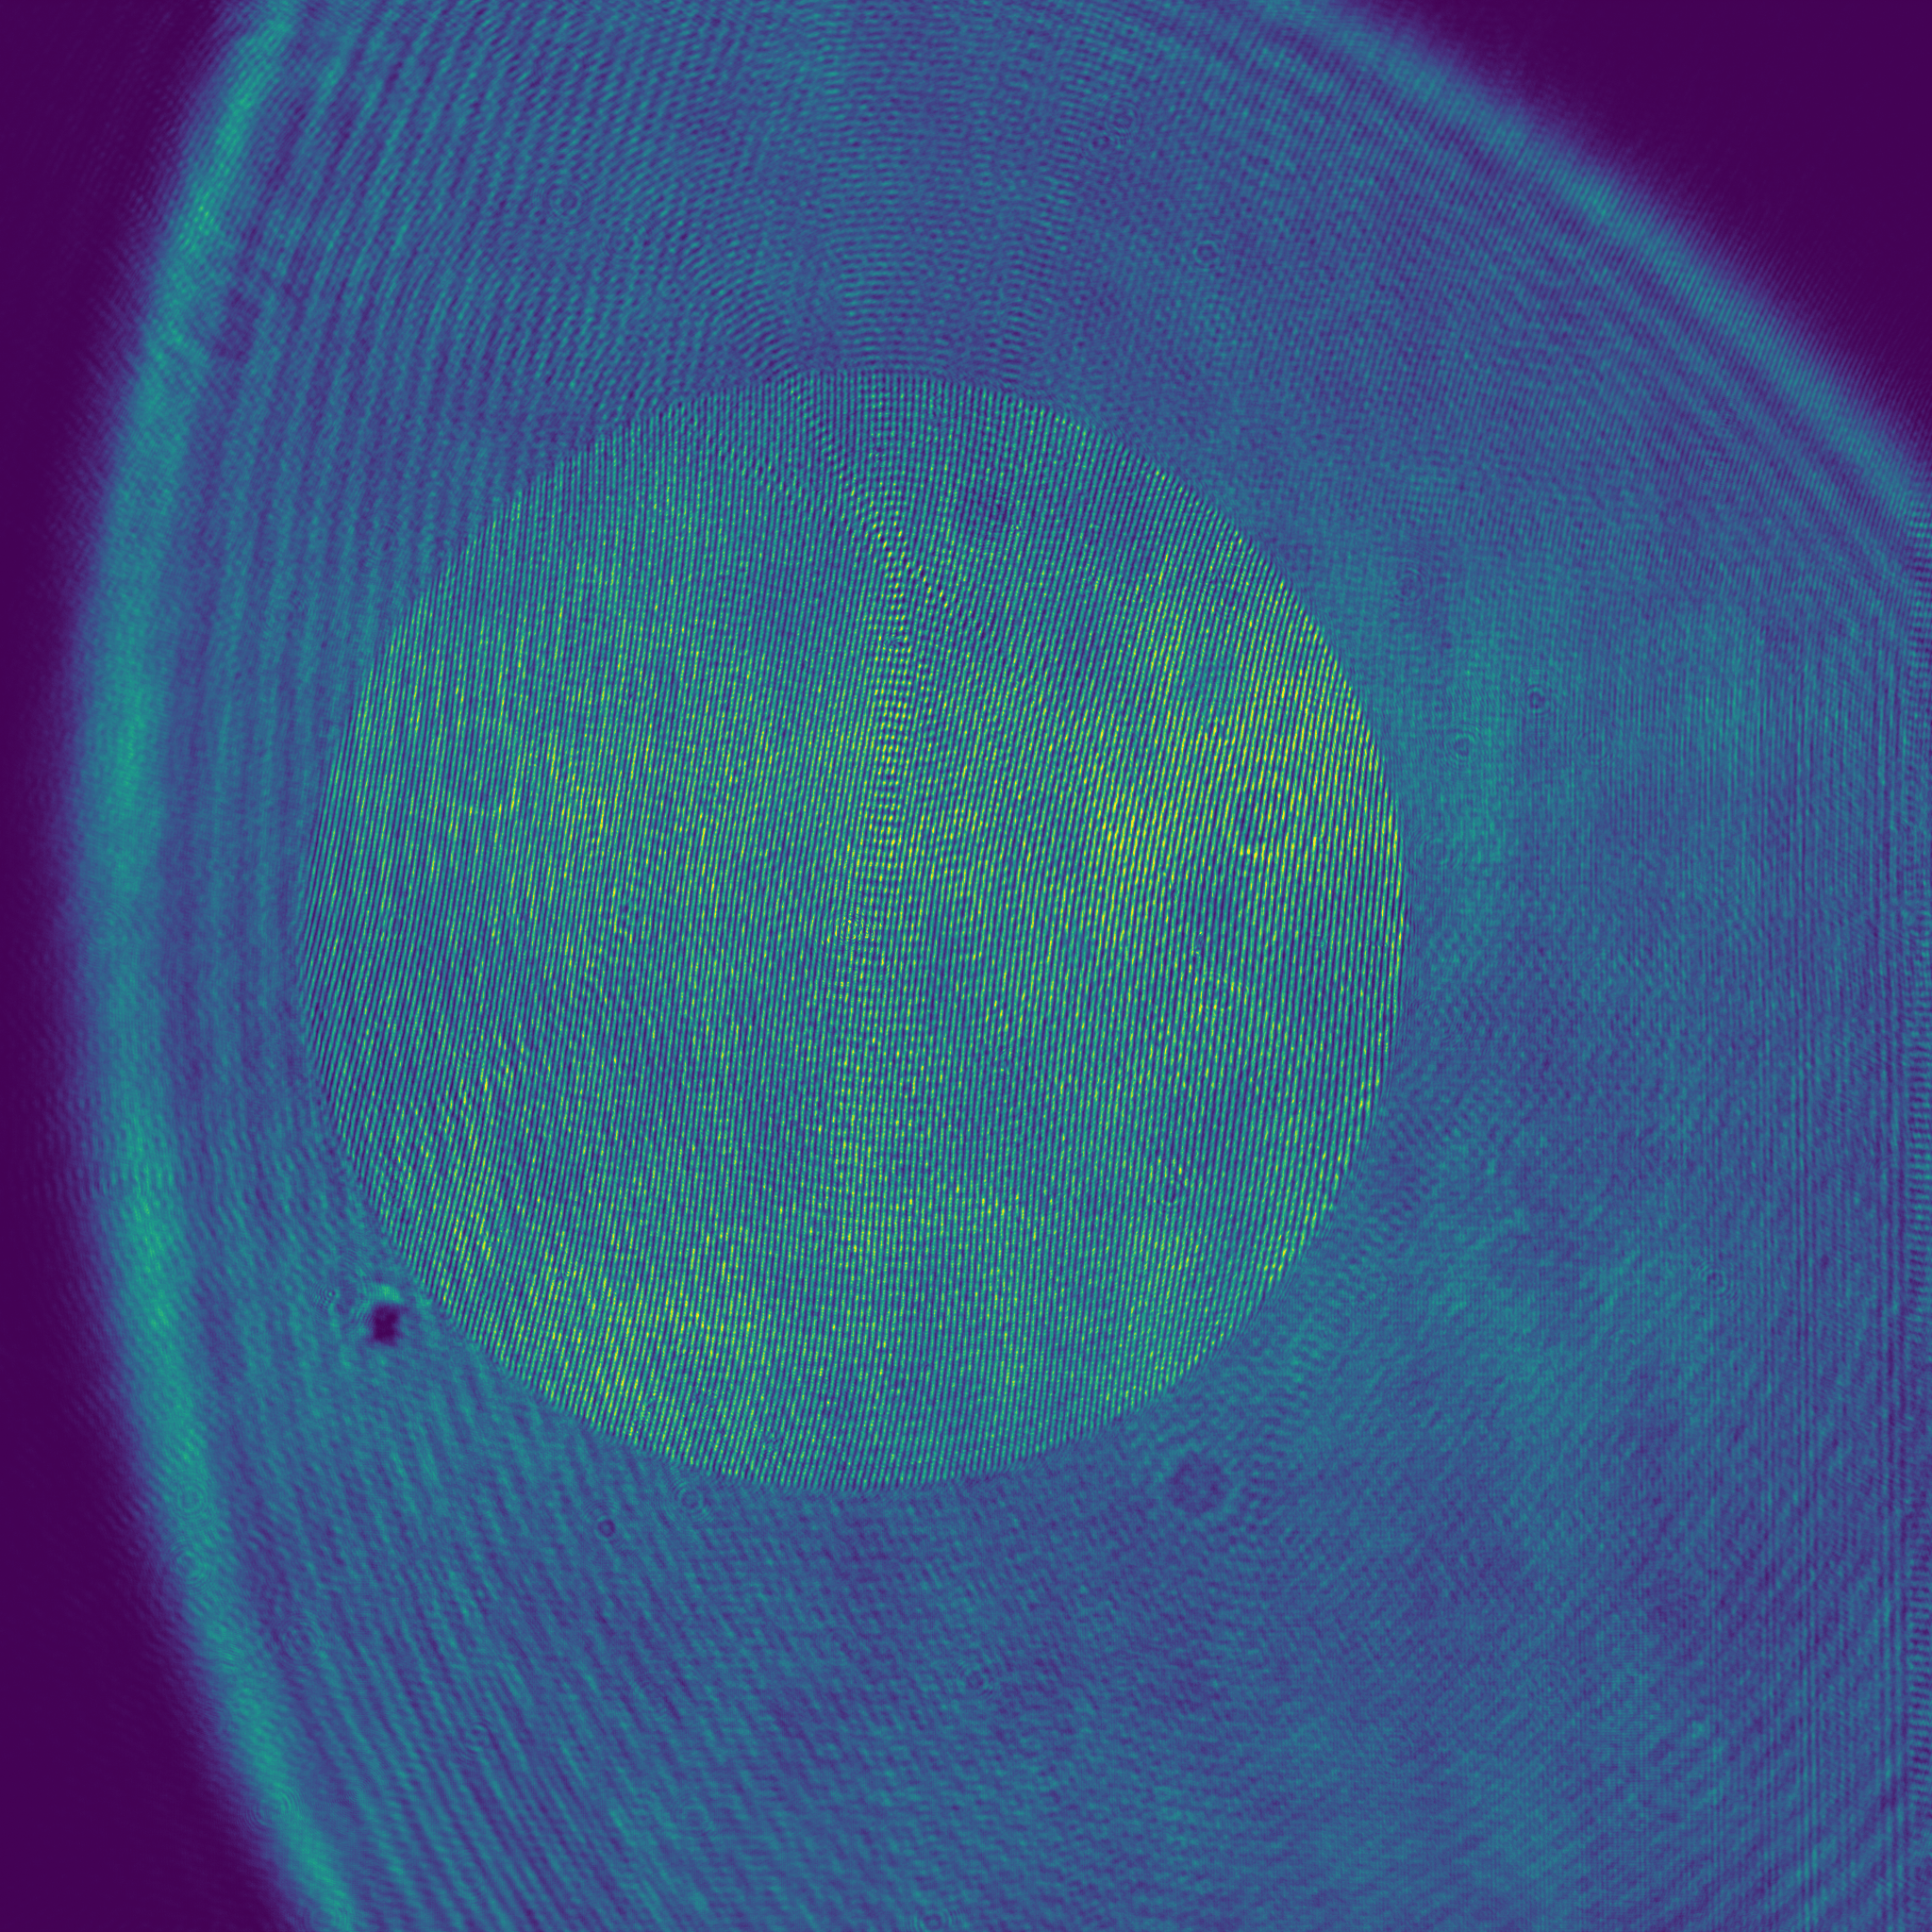
\includegraphics[width=1\linewidth, scale=0.5]{images/puw_inteferogram.png}
		\caption{}
		\label{fig:puw_inteferogram}
	\end{subfigure}
	\begin{subfigure}{0.23\textwidth}
		\centering
		\includegraphics[width=1\linewidth, scale=0.5]{images/puw_inteferogram_cropped.png}
		\caption{}
		\label{fig:puw_inteferogram_cropped}
	\end{subfigure}
	\begin{subfigure}{0.23\textwidth}
		\centering
		\includegraphics[width=1\linewidth, scale=0.5]{images/puw_mask.png}
		\caption{}
		\label{fig:puw_mask}
	\end{subfigure}
	\begin{subfigure}{0.23\textwidth}
		\centering
		\includegraphics[width=1\linewidth, scale=0.5]{images/puw_data_masked.png}
		\caption{}
		\label{fig:puw_data_masked}
	\end{subfigure}
	
	\begin{subfigure}{0.23\textwidth}
		\centering
		\includegraphics[width=1\linewidth, scale=0.5]{images/puw_data_fftshift.png}
		\caption{}
		\label{fig:puw_data_fftshift}
	\end{subfigure}
	\begin{subfigure}{0.23\textwidth}
		\centering
		\includegraphics[width=1\linewidth, scale=0.5]{images/puw_tukey_window.png}
		\caption{}
		\label{fig:puw_tukey_window}
	\end{subfigure}
	\begin{subfigure}{0.23\textwidth}
		\centering
		\includegraphics[width=1\linewidth, scale=0.5]{images/puw_fringes_tukey.png}
		\caption{}
		\label{fig:puw_fringes_tukey}
	\end{subfigure}
	\begin{subfigure}{0.23\textwidth}
		\centering
		\includegraphics[width=1\linewidth, scale=0.5]{images/puw_new_fringe_fft.png}
		\caption{}
		\label{fig:puw_new_fringe_fft}
	\end{subfigure}
	
	\begin{subfigure}{0.23\textwidth}
		\centering
		\includegraphics[width=1\linewidth, scale=0.5]{images/puw_new_fringe_fft_centre_blocked.png}
		\caption{}
		\label{fig:puw_new_fringe_fft_centre_blocked}
	\end{subfigure}
	\begin{subfigure}{0.23\textwidth}
		\centering
		\includegraphics[width=1\linewidth, scale=0.5]{images/puw_fft_filter.png}
		\caption{}
		\label{fig:puw_fft_filter}
	\end{subfigure}
	\begin{subfigure}{0.23\textwidth}
		\centering
		\includegraphics[width=1\linewidth, scale=0.5]{images/puw_new_fringe_order1.png}
		\caption{}
		\label{fig:puw_new_fringe_order1}
	\end{subfigure}
	\begin{subfigure}{0.23\textwidth}
		\centering
		\includegraphics[width=1\linewidth, scale=0.5]{images/puw_order1_roll.png}
		\caption{}
		\label{fig:puw_order1_roll}
	\end{subfigure}
	
	\begin{subfigure}{0.23\textwidth}
		\centering
		\includegraphics[width=1\linewidth, scale=0.5]{images/puw_complex_phase.png}
		\caption{}
		\label{fig:puw_complex_phase}
	\end{subfigure}
	\begin{subfigure}{0.23\textwidth}
		\centering
		\includegraphics[width=1\linewidth, scale=0.5]{images/puw_phaseorder1.png}
		\caption{}
		\label{fig:puw_phaseorder1}
	\end{subfigure}
	\begin{subfigure}{0.23\textwidth}
		\centering
		\includegraphics[width=1\linewidth, scale=0.5]{images/puw_phaseorder1mask}
		\caption{}
		\label{fig:puw_phaseorder1mask}
	\end{subfigure}
	\begin{subfigure}{0.23\textwidth}
		\centering
		\includegraphics[width=1\linewidth, scale=0.5]{images/puw_unwrapped_phase.png}
		\caption{}
		\label{fig:puw_unwrapped_phase}
	\end{subfigure}
	\caption{A visualisation of the stages of the phase unwrap workflow. (a) Captured interferogram (b) Interferogram cropped to region of interest (ROI) (c) Circular mask (d) ROI isolated (e) ROI quadrant shifted (ROI-qs) (f) 2-D tukey window mask (g) ROI-qs with tukey mask applied (h) Fast Fourier transform (FFT) of (g), log scaled (i) Fourier transform with the central spatial frequencies masked, log scaled (j) 2-D sine squared mask centred on the position of spatial frequencies encoding the phase information (k) The original Fourier transform, (h), with the sine squared mask applied (l) Phase encoding spatial frequencies rolled to the central position (m) Inverse FFT of the phase encoding spatial frequencies (n) Inverse FFT transformed into a phase map (o) Phase map masked to isolate ROI (p) Phase map unwrapped to remove 2$\pi$ discontinuities}
	\label{fig:phase_unwrap_workflow}
\end{figure*}

Having performed the FFT (\ref{fig:puw_new_fringe_fft}), an array described by Equation~\ref{eq:I_fourier} is obtained. A selection of the central spatial frequencies are masked (\ref{fig:puw_new_fringe_fft_centre_blocked}), primarily to mask out the central spatial frequency which represents the mean intensity and has an amplitude orders of magnitude larger than any other spatial frequency. The spatial frequencies which now have the highest amplitudes correspond to both $\boldsymbol{C}(u,v)$ and $\boldsymbol{C}^{*}(u,v)$. One of the aforementioned amplitude peaks is located and a bandpass filter described by $\sin^{2}(x,y)$ is constructed (\ref{fig:puw_fft_filter}) centred on the spatial frequency location of this amplitude peak. As previously noted, the Fourier transform of the interferogram is symmetrical around the central spatial frequency. So, it doesn't matter which of the two peaks this filter is centred on since they encode the same information. This bandpass filter is then applied to the FFT of the interferogram (\ref{fig:puw_new_fringe_order1}) and these spatial frequencies are then rolled to the central spatial frequency position (\ref{fig:puw_order1_roll}). This successfully filters $\boldsymbol{A}(u,v)$ and $\boldsymbol{C}^{*}(u,v)$, isolating $\boldsymbol{C}(u,v)$ as desired.

The array corresponding to $\boldsymbol{C}(u,v)$ is inverse Fourier transformed to yield $c(x,y)$ (\ref{fig:puw_complex_phase}). This is then converted to a phase map by performing the calculation in Equation~\ref{eq:phase} (\ref{fig:puw_phaseorder1}) and the mask in Figure~\ref{fig:puw_mask} is applied again to mask out any spurious noise outside the ROI. Due to the periodic nature of trigonometric functions, this phase map is wrapped around $-\pi$ and $\pi$. An 2D  algorithm is used to unwrap the phase map and yield a phase map similar to Figure~\ref{fig:puw_unwrapped_phase} is obtained.\cite{herraez2002fast} Other than determining the appropriate ROI, this workflow is entirely automated and requires no user input. 

This automation does have a drawback. The location of the phase component of the Fourier transform is determined by finding the maximum intensity in the data represented by Figure~\ref{fig:puw_new_fringe_fft_centre_blocked} and then performing a number of centre of mass calculations to find the `true' centre of the phase component. However, this `true' centre may still be incorrect by a few pixels. This leads to an artificial introduction of tip and/or tilt in the final wavefront and this artificial tip/tilt cannot be separated from the true tip/tilt. Therefore, this phase unwrapping implementation cannot be said to be sensitive to tip or tilt. However, since tip and tilt (along with piston) is not considered to be a true optical aberration, this seems a small price to pay for a fully automated phase unwrapping workflow.

\subsubsection{Characterisation}

A potential problem with the automated calibration routine is a lack of feedback. This issue arises from a number of places including the fact that some parameters, such as the number of steps used to calibrate each actuator and the threshold used in the SVD pseudo-inversion, are chosen somewhat arbitrarily, the approximate nature of the pseudo-inverse, and discretisation errors in the measuring of Zernike modes. It is therefore necessary to have some measure of how well the deformable mirror is able to recreate desired Zernike modes. This process is called characterisation. The process involves applying a fixed amplitude of a single Zernike mode to the mirror, measuring the Zernike mode applied and comparing the amplitude to that supposedly applied. An automated implementation of this process is present in Microscope-AOtools with the results returned to the user for interrogation. Figure~\ref{fig:characterisation_workflow} shows a flowchart of this method in Microscope-AOtools. The background wavefront distortion is measured and the Zernike mode amplitudes are measured. These are subtracted from the Zernike modes measured with deformations applied to the mirror to give an accurate assessment of the shape of the deformable mirror. 

\begin{figure}[h]
	\centering
	\includegraphics[width=0.4\textwidth, scale=0.5]{./images/characterisation_workflow.jpg}
	\caption{Flowchart depicting the process for characterising a deformable mirror as implemented in Microscope-AOtools}
	\label{fig:characterisation_workflow}
\end{figure}

In an ideal situation, where the control matrix provided a perfect linear map from Zernike mode amplitudes to DM actuator positions, we would expect to see a characterisation assay like that in Figure~\ref{fig:characterisation_assay_ideal}, where only the desired Zernike mode is applied. In practice, the mirror is better at recreating particular Zernike modes than others and the coupled nature of the actuators means that small amplitudes of other Zernike modes are also present. The drop in quality of recreation becomes pronounced at high order Zernike modes since a deformable mirror (in this case, an Alpao-69 deformable mirror) lacks the adequate degrees of freedom to accurately recreate complex Zernike modes.

\begin{figure}[h]
	\centering
	\begin{subfigure}{0.25\textwidth}
		\includegraphics{./images/characterisation_assay_ideal.png}
		\caption{}
		\label{fig:characterisation_assay_ideal}
	\end{subfigure}
	\begin{subfigure}{0.25\textwidth}
		\includegraphics{./images/characterisation_assay_real.png}
		\caption{}
		\label{fig:characterisation_assay_real}
	\end{subfigure}
	\begin{subfigure}{0.4\textwidth}
		\includegraphics{./images/characterisation_assay_real_diag_and_avg.png}
		\caption{}
		\label{fig:characterisation_assay_ideal_diag_and_avg}
	\end{subfigure}
	\caption{(a) An ideal characterisation assay, measuring the recreation accuracy of 68 Zernike modes with applied amplitude of 1 for each (b) A realistic characterisation assay obtained from a calibrated Alpao-69 actuator DM, measuring the recreation accuracy of 68 Zernike modes with applied amplitude of 1 for each (c) Plot of the amplitudes desired Zernike modes i.e. the diagonal values of the characterisation assay. Individual values plotted as well as a shifting average (the average of the current mode and all preceding modes)}
	\label{fig:characterisation_assay_results}
\end{figure}

Whether a calibration routine is considered a 'success' depends on the requirements of the DM within the system. Taking the characterisation assay shown in Figure~\ref{fig:characterisation_assay_real}, if success criteria for the DM is to be able correct for the first 20 Zernike modes with an 80\% accuracy, the calibration routine could be considered successful based on the characterisation assay generated. However, if the success criteria were for 90\% recreation accuracy for the first 30 Zernike modes, then the calibration routine would not have been successful and would need to be performed again, likely with altered parameters. It is left to the user to determine the success criteria for the DM calibration but Microscope-AOtools provides the tool necessary to determine whether they have been satisfied or not.

\section{Use Case Methods}

\subsection{Direct Wavefront Sensing Correction}

The applications for aberration correction using direct wavefront sensing have been well documented. However, the wavefront is measured (interferometry, Shack-Hartmann wavefront sensor, fluorescent guide star, etc) being able to measure the Zernike modes present and correct for them is a useful method to have for correcting both system and sample induced aberrations. Microscope-AOtools implements a correction method where the wavefront if observed directly. This is not a complex method. The workflow is shown in Figure~\ref{fig:direct_wavefront_flattening_workflow}. The wavefront is obtained through whatever direct wavefront sensing method has been implemented and selected, a number of Zernike modes determined by the user are fitted to the wavefront, an equal and opposite magnitude of these modes are applied to the DM. The RMS wavefront error is then obtained. This process repeats until $N$ iterations have been performed and the RMS wavefront error is below a user defined error threshold, $\delta$.

\begin{figure}[h]
	\centering
	\includegraphics[width=0.55\textwidth, scale=0.5]{./images/direct_wavefront_flattening_workflow.png}
	\caption{Flowchart depicting the process for flattening directly measured wavefront as implemented in Microscope-AOtools}
	\label{fig:direct_wavefront_flattening_workflow}
\end{figure}

In an ideal setup with a perfect control matrix, this process would only need to be performed once. However, as we have already discussed, the control matrices generated for any setup are never `perfect'. Therefore, one iteration of this method would correct the aberrations to an extent, but it would leave residual aberrations. It is necessary to perform this process for a number of iterations to ensure the optimal wavefront is obtained. 

Figure~\ref{fig:direct_wavefront_correction} shows the results of one such wavefront correction. The wavefront was obtained by interferometry and, due to previously mentioned insensitivity to tip and tilt and since piston, tip and tilt are not true optical aberrations, Zernike modes 4-69 (using Noll indices) were corrected over 10 iterations. The RMS phase errors in Figures~\ref{fig:aberrated_wavefront_defocus_ptt_rmv_crop_phase_only} and \ref{fig:flattened_wavefront_10it} are 28.58368 radians and 3.11921 radians respectively. Figure~\ref{fig:zernike_modes_to_show_flattening} shows the Zernike mode amplitudes before and after correction. Clearly there is some over-correction in the defocus mode (Noll index 4) in particular which is visible in Figure~\ref{fig:flattened_wavefront_10it}. The dots visible are the physical location of the actuators on the DM and represent a limiting factor in how flat the DM surface can actually be. 

\begin{figure}[h]
	\centering
	\begin{subfigure}{0.33\textwidth}
		\includegraphics[scale=2]{./images/aberrated_wavefront_defocus_ptt_rmv_crop_phase_only.png}
		\caption{}
		\label{fig:aberrated_wavefront_defocus_ptt_rmv_crop_phase_only}
	\end{subfigure}
	\begin{subfigure}{0.425\textwidth}
		\includegraphics[scale=2]{./images/flattened_wavefront_10it_ptt_rmv_phase_colorbar1.png}
		\caption{}
		\label{fig:flattened_wavefront_10it}
	\end{subfigure}

	\begin{subfigure}{0.5\textwidth}
		\includegraphics[scale=2]{./images/zernike_amps_before_and_after_10it_modes_4to69.png}
		\caption{}
		\label{fig:zernike_modes_to_show_flattening}
	\end{subfigure}
	\caption{(a) An aberrated wavefront (b) A wavefront after 10 iterations of correction (c) The Zernike mode amplitudes measured in the aberrated (red) and corrected (blue) wavefronts (a) - (b) are all presented on the same colorscale (in radians) and were obtains via interferometry}
	\label{fig:direct_wavefront_correction}
\end{figure}

Similar to the calibration routine, the success criteria for direct wavefront correction is left to the user. For direct wavefront corrections preformed on samples, the preference may be to obtain the best possible correction within \textit{N} iterations. For system aberration corrections using an interferometer, where photo bleaching is not an issue, is may be preferable to simply set a minimum error and continue to iterate until this threshold is reached. Microscope-AOtools implements both options to ensure generalisability.

\subsection{Sensorless Correction}

In many biological applications, direct wavefront sensing is not possible and so we rely on wavefront sensorless techniques to determine the best correction to apply. The generalised methodology for this is shown in Figure~\ref{fig:sensorless_correction_method}. Some metric, $S$, which gives some useful measure of the image quality is chosen. For each Zernike modes, $Z_{i}$, a number of amplitudes of that mode, $a_{j}$, are applied and an image of the sample obtained for each. The image quality of each image, $S_{j}$ is obtained. Assuming that $S$ is a function of $a$, fitting a Gaussian function to the $S_{j}$ values yields an Zernike mode amplitude, $a_{max}$, which should, theoretically, yield the best image quality, $S_{max}$. 

\begin{figure}[h]
	\centering
	\includegraphics[width=1\textwidth,scale=0.5]{./images/sensorless_aberration_fitting_w_images.png}
	\caption{Principle of sensorless adaptive optics correction. For each Zernike mode, $Z_i$, images of the sample with different amplitudes of the $i$-th Zernike mode are obtained. A value of the image quality metric, $S$, is obtained for each (blue dots). A Gaussian function is then fitted to these values and the amplitude, $a$ corresponding to the maximum image quality, $S_{max}$, is obtained (green dot). The inset images are Drosophila Neuro-muscular Junction with various amplitudes of spherical aberration present.}
	\label{fig:sensorless_correction_method}
\end{figure}

The complexity of sensorless adaptive optics correction lies in selecting the best image quality metric. There have been numerous metrics developed which have been shown to be effective on certain sample types or imaging modalities.\cite{burke2015adaptive,booth2002adaptive,fienup2003aberration,debarre2008adaptive} In order for an adaptive optics implementation to be considered generalised, it should not be tied to a particular sample type or imaging modality. For this reason, Microscope-AOtools offers a range of image quality metrics, all located in the \textit{aoMetrics.py}, and which we will discuss shortly.  

Unlike the calibration, characterisation and direct wavefront sensing techniques, an automated sensorless adaptive optics routine is not implemented in Microscope-AOtools. This is a design choice since to do so would mean giving AOtools control over multiple pieces of hardware such as imaging cameras, light sources, etc. Python Microscope already fulfils this role and so we decided to not reimplement work already done elsewhere. Figure~\ref{fig:sensorless_correction_workflows} shows the options for sensorless correction workflows.

Applying the $j$-th amplitudes of the $i$-th Zernike modes is a method present in Microscope-AOtools by passing a 1-D array of $N$ Zernike mode amplitudes to the \lstinline|set_phase| function. The user has to set up their system to take images after each array of Zernike mode amplitudes is applied. The two main decisions a user has to make when constructing their sensorless correction workflow are when to measure the image quality metric and when to apply the corrections for each Zernike modes. In the workflows in Figure~\ref{fig:sensorless_correction_workflow_1} and \ref{fig:sensorless_correction_workflow_2} the correction is calculated for one Zernike mode and then applied before correcting the next Zernike mode. If the order of correction is chosen well so that the modes with the largest amplitudes are corrected first, this can have significant benefit over the workflow shown in Figure~\ref{fig:sensorless_correction_workflow_3}. Measuring the image quality metrics for single images, a stack of $M$ images for one Zernike mode or $NM$ images for all Zernike modes are all methods which Microscope-AOtools has as the functions \lstinline|measure_metric|, \lstinline|correct_sensorless_single_mode| and \lstinline|correct_sensorless_all_modes| respectively. In the case of the latter two the function returns the best Zernike mode amplitude for the single Zernike mode and all Zernike modes measured respectively.

\begin{figure}[h]
	\begin{subfigure}{0.425\textwidth}
		\includegraphics[scale=0.55]{./images/sensorless_correction_workflow_1.jpg}
		\caption{}
		\label{fig:sensorless_correction_workflow_1}
	\end{subfigure}
	\begin{subfigure}{0.425\textwidth}
		\includegraphics[scale=0.55]{./images/sensorless_correction_workflow_2.jpg}
		\caption{}
		\label{fig:sensorless_correction_workflow_2}
	\end{subfigure}
	
	\centering
	\begin{subfigure}{0.425\textwidth}
		\includegraphics[scale=0.55]{./images/sensorless_correction_workflow_3.jpg}
		\caption{}
		\label{fig:sensorless_correction_workflow_3}
	\end{subfigure}
	\caption{Flowcharts depicting the sensorless correction routine options (a) An image for each amplitude of the $i$-th Zernike mode is taken and the image quality metric is immediately evaluated. Once all the images for the $i$-th Zernike mode have been taken, the best Zernike amplitude is found as described in Figure~\ref{fig:sensorless_correction_method} and applied (b) All $M$ images are taken, then the quality metric is obtained for all $M$ images, the best Zernike amplitude is found and applied (c) All the images for all the $N$ Zernike modes are obtained with no correction applied in between modes. The image quaility metric then measured for every image and the best amplitude for each Zernike mode is found. The correction for all modes is applied simultaneously at the end of the workflow.}
	\label{fig:sensorless_correction_workflows}
\end{figure}

\subsubsection{Contrast Metric}

Signal-to-noise contrast is perhaps the most basic measure of image quality. Indeed, it is closely related to resolution. A microscope may have a theoretically achievable resolution but if the signal-to-noise contrast is poor then the effective resolution may be considerably lower. The contrast metric implemented in Microscope-AOtools is defined as:

\begin{equation}\label{eq:contrast_metric}
S = \frac{\sum\limits_{j=N-M}^{N}{I'_{j}}}{\sum\limits_{j=1}^{M}{I'_{j}}}
\end{equation}

Where $I'$ is the original image, $I$, flattened into a 1-D array and ascending ordered, $N$ is the total number of pixels and $M$ is some user defined number of pixels. Simply, $S$ is the ratio of the $M$-th highest pixel values to the $M$-th lowest pixel values. This contrast metrics is useful as a first approximation where users might not be clear which metric would be best for their sample/imaging modality. However, it vulnerable to samples which are susceptible to rapid photobleaching or some other phenomenon which decreases the signal without affecting the noise level. 

\subsubsection{Second Moment Metric}

The Second Moment of the Fourier transform was a metric which was developed for single-molecule switching microscopy, designed to be insensitive to the intensity and number of emitters present in a sample.\cite{burke2015adaptive} It was defined thusly:

\begin{equation}\label{eq:second_moment_metric_old}
S = \frac{\sum\limits_{n,m}{\mu_{n,m}\hat{I}_{n,m}(n'^{2} + m'^{2})}}{\sum\limits_{n,m}{\hat{I}_{n,m}}}
\end{equation}

Where $\hat{I}_{n,m}$ is the discrete Fourier transform of the image, $n' = n - \frac{N-1}{2}$, $m' = m - \frac{M-1}{2}$ and $n$ and $n$ are coordinates ranging from $0$ to $N-1$ or $M-1$, respectively, where $N$ and $M$ are the number of pixels along each dimension of the image. The
function $\mu_{n,m}$ is a circular mask, given by:

\begin{equation}\label{eq:circular_mask}
\mu_{n,m} = 
\begin{cases}
1, & \sqrt{n'^{2} + m'^{2}} \le w\\
0 & \sqrt{n'^{2} + m'^{2}} > w\\ 
\end{cases}
\end{equation}

Where $w$ was a radius defined as the size of the field of view of the image divided by the expected resolution of the wide-field imaging system, assumed to be approximately the Abbe diffraction limit. 

The Microscope-AOtools implementation of this metric makes two minor amendments. Firstly, $w$ is explicitly set as the Abbe diffraction limit, $\frac{1.22 \lambda}{2 NA}$. Secondly, an attenuation factor was added to the ramp factor, $(n'^{2} + m'^{2})$. This ramp factor amplified the highest spatial frequencies. However, the spatial frequencies close to the reciprocal of the Abbe limit are rarely filled in imaging systems and often primarily composed of noise. Amplifying these spatial frequencies had a tendency to bias the final $S$ value based on the noise values. Therefore, the Microscope-AOtools implementation of the Second Moment metric is defined as:

\begin{equation}\label{eq:second_moment_metric}
S = \frac{\sum\limits_{n,m}{\mu_{n,m}\hat{I}_{n,m}\omega(n'^{2} + m'^{2})}}{\sum\limits_{n,m}{\hat{I}_{n,m}}}
\end{equation}

Where the attenuation factor, $\omega$, is defined as:

\begin{equation}\label{eq:attenuation_mask}
\omega = 1 - e^{\frac{\sqrt{n'^{2} + m'^{2}}}{w}-1}
\end{equation}

Where $n'$,$m'$ and $w$ are all defined as before. This attenuation factor does become negative at $n'^{2} + m'^{2} > w$, however since $\mu_{n,m}$ is $0$ at this point, this is irrelevant. Figure~\ref{fig:second_moment_combine_mask_w_cross_section} shows the combined effect of $\mu_{n,m}\omega(n'^{2} + m'^{2})$. Combined, they amplify the middle-high spatial frequencies while the low and very high spatial frequencies (close to $w$) are suppressed, preventing bias due to spurious noise in the Fourier transform. Therefore, the Second Moment metric is still insensitive to the intensity and number of emitters present in a sample as well as being more robust against noise.

\begin{figure}[h]
	\begin{subfigure}{0.4\textwidth}
		\includegraphics[scale=1]{./images/second_moment_combine_mask.png}
		\caption{}
		\label{fig:second_moment_combine_mask}
	\end{subfigure}
	\begin{subfigure}{0.41\textwidth}
		\includegraphics[scale=1]{./images/second_moment_combine_mask_cross_section.png}
		\caption{}
		\label{fig:second_moment_combine_mask_cross_section}
	\end{subfigure}
	\caption{(a) A visualisation of the combined attenuation mask of the Second Moment of the Fourier transform, $\mu_{n,m}\omega(n'^{2} + m'^{2})$ (b) a cross section of the combined attenuation mask showing that the middle-high spatial frequencies are still amplified while the very high spatial frequencies (close to $w$) are suppressed. The magnitude of amplification is not show as this is proportional to the image shape and therefore not meaningful.}
	\label{fig:second_moment_combine_mask_w_cross_section}
\end{figure}

\subsubsection{Fourier Metric}

Utilising Fourier space information as a measure of image quality is beneficial, particularly for imaging modalities which rely on spatial frequency information such as structured illumination microscopy (SIM). In a noise-free system, the Fourier transform of an image would only contain spatial frequencies which corresponded to information in the original image. A greater number of these spatial frequencies would correspond to a sharper image. Microscope-AOtools implements a metric to extract the number of signal spatial frequencies and thereby quantify the sharpness of the image, defined as:

\begin{equation}\label{eq:Fourier_metric}
S = \sum\limits_{n,m}{\mu_{n,m}\tau_{n,m}}
\end{equation}

Where $\mu_{n,m}$ is defined the same as in Equation~\ref{eq:circular_mask} and $\tau_{n,m}$ is a binary mask defined as:

\begin{equation}\label{eq:noise_threshold_mask}
\tau_{n,m} = 
\begin{cases}
0, & \vline \hat{I}_{n,m} \vline^2 < \delta\\
1 & \vline \hat{I}_{n,m} \vline^2 \ge \delta\\ 
\end{cases}
\end{equation}

Where $\delta$ is a threshold defined as:

\begin{equation}\label{eq:noise_threshold}
\delta = \alpha\langle \vline \hat{I}_{l,k} \vline^2 \rangle
\end{equation}

Where $l$ \& $k$ are the coordinates where $\mu_{n,m} = 0$, $\alpha$ is a user defined amplification factor which sets the threshold relative to the mean of the noise in the Fourier transform and $\hat{I}_{n,m}$ is, as before, the discrete Fourier transform of the image. Simply, this Fourier based metric counts the number of spatial frequencies with power above an approximation of the noise floor. 

We can be sure that the $\langle \vline \hat{I}_{l,k} \vline^2 \rangle$ yields the mean value of the noise power because $l$ \& $k$ are the coordinates where $\mu_{n,m} = 0$, i.e. the mean of the spatial frequencies outside of the Abbe limit of the microscope. Since these spatial frequencies cannot contain any signal power, whatever power they contain must be noise. The amplification factor, $\alpha$, is present since setting the threshold to simply be the mean of the noise would mean that $\tau_{n,m}$ still captured some noisy spatial frequencies. We have found an $\alpha = 1.125$ is sufficient to suppress the noise-dominated spatial frequencies without suppressing the signal-dominated spatial frequencies. 

This Fourier metrics offers a robust way to maximise the spatial frequency content in an image whilst also being insensitive of the image intensity and extremely robust against noise in both the original image and in the Fourier domain.

\subsubsection{Fourier Power Metric}

Whilst the Fourier metric described previously is a useful and robust metric for SIM and other spatial frequency-dependent imaging modalities, it does trade some useful information for its robustness. In particular, by simply counting the number of signal-dominated spatial frequencies it ignores the information contained in the power of those spatial frequencies. Microscope-AOtools therefore also implements a variant of the Fourier metric which takes the spatial frequency powers into account defined as:

\begin{equation}\label{eq:Fourier_power_metric}
S = \sum\limits_{n,m}{\mu_{n,m}\tau_{n,m}\omega'\vline \hat{I}_{n,m} \vline^2}
\end{equation}

Where $\mu_{n,m}$ and $\tau_{n,m}$ have their previous definitions found in Equations~\ref{eq:circular_mask} and \ref{eq:noise_threshold_mask}, $\hat{I}_{n,m}$ is still the discrete Fourier transform and $\omega'$ is a modified version of Equation~\ref{eq:attenuation_mask} defined as:

\begin{equation}\label{eq:attenuation_mask_norm_and_scaled}
\omega' = \beta \vline \omega(n'^{2} + m'^{2}) \vline
\end{equation}

Where $\omega$, $n'$ and $m'$ are defined as before and $\beta$ is a user defined normalisation factor. $\mu_{n,m}\omega'$ creates a similar attenuation mask to the one shown in Figure~\ref{fig:second_moment_combine_mask_w_cross_section} except, whereas the maximum amplification of the mask shown in the Figure~\ref{fig:second_moment_combine_mask_w_cross_section} is proportional to image size, the attenuation mask is first normalised to have a range $[0,1]$ and then scaled to the normalisation factor, $\beta$.

This Fourier Power metric is sensitive to power being moved to and from lower spatial frequencies to higher spatial frequencies, even if no new spatial frequencies are raised to be above or below the noise threshold, $\delta$. However, due to Parseval's theorem, this does also mean that the Fourier Power metric is sensitive to the amplitude of original image. This means that it may not be suitable for samples which suffer from rapid photobleaching as this is likely bias the correction results towards Zernike mode measurements taken first. For relatively photo-stable dyes this does not present a serious issue.

\subsection{IsoSense}

For samples or imaging modalities which rely on structural information, anisotropies in the structures present can bias the corrections produced. There has recently been a technique developed to overcome this issue; IsoSense.\cite{vzurauskas2019isosense} It relies on producing spatially structured light in order to fill empty sections of the Fourier transform. If a spatial light modulator (SLM) is defined and present in the optical setup, Microscope-AOtools incorporates the methods necessary to apply the spatially structured illumination necessary to utilise this technique. Figure~\ref{fig:isosense_visualisation} shows both the structured illumination pattern and the location of the beams in Fourier space. The location of these beams are: $(0,0)$, $(0,\gamma w)$, $(0,-\gamma w)$, $(\gamma w, 0)$, $(-\gamma w, 0)$, $(\frac{\gamma w}{2}, \frac{\gamma w}{2})$, $(-\frac{\gamma w}{2}, \frac{\gamma w}{2})$, $(\frac{\gamma w}{2}, -\frac{\gamma w}{2})$, $(-\frac{\gamma w}{2}, -\frac{\gamma w}{2})$. $w$ is the Abbe diffraction limit as before and $\gamma$ is a user defined fill fraction. This fill fraction is added because, depending on the sample and the severity of aberration, the location of the beams in Fourier space (corresponding to the area of the Fourier spectrum which needs to be filled) may change. Placing these beams is an skill for more advanced users, however the implementation in Microscope-AOtools means this is the only complexity a user has to worry about.

\begin{figure}[h]
	\centering
	\begin{subfigure}{0.4\textwidth}
		\includegraphics{./images/isosense_visualisation_real.png}
		\caption{}
		\label{fig:isosense_visualisation_real}
	\end{subfigure}
	\begin{subfigure}{0.4\textwidth}
		\includegraphics{./images/isosense_visualisation_ft.png}
		\caption{}
		\label{fig:isosense_visualisation_ft}
	\end{subfigure}
	\caption{(a) A simulated IsoSense pattern created with a 4-beam interference (b) A diagram of a 4 beam interference pattern in Fourier space. The diagonal axis and the horizontal/vertical axis have $\frac{1}{2}$ and $\frac{1}{4}$ of the intensity of the central beam respectively.}
	\label{fig:isosense_visualisation}
\end{figure}

\section{Discussion}

In order for Microscope-AOtools to be considered generalised, a user should be able to take an arbitrary deformable mirror in an arbitrary set-up, calibrate it and use it on an arbitrary sample type in an arbitrary imaging modality. Since Microscope-AOtools relies on Python Microscope, it can only implement deformable mirrors which Python Microscope can control. However, adding new devices to Python Microscope is relatively simple. Refer to Python Microscope (\url{https://www.python-microscope.org/}) for more details. Currently, all that is required to set-up an arbitrary Python Microscope deformable mirror in an arbitrary set-up is for there to be an interferometer present. If one is not present, constructing one is relatively simple. The calibration and characterisation routines can then be performed with minimal effort. 

It has already been noted that the only wavefront sensing currently implemented in Microscope-AOtools is interferometry. It is therefore not unreasonable to question the claims of generalisability. Here we would like to draw a distinction between `universal' and `generalised'. For Microscope-AOtools to be `universal' it would have to implement every wavefront sensing technique and be able to swap between them easily. However, in order for Microscope-AOtools to be `generalised' it need only be designed so that the workflow can accept any wavefront sensing technique. This is the case with Microscope-AOtools. 

Figures~\ref{fig:Ith_actuator_calibration_workflow}, \ref{fig:characterisation_workflow} and \ref{fig:direct_wavefront_flattening_workflow} show the key workflows which require phase images. In every instance this is done with a single call: \lstinline|unwrap_method[self.phase_method](image)|. \lstinline|unwrap_method| is a dictionary of phase retrieval functions with the attribute \lstinline|self.phase_method| governing which method to use. All that is required to add a new phase retrieval method is to write the function which performs only that operation on an input image and returns a phase image, adding that function to the \lstinline|unwrap_method| dictionary and the appropriate checks to \lstinline|check_unwrap_conditions| function. So, although Microscope-AOtools is not `universal' it is `generalised' since any novel phase retrieval method can be added to the workflow without having to recreate any other part of the calibration, characterisation or wavefront flattening workflows. 

Microscope-AOtools is further generalised since it has methods for manually setting a control matrix to be used. This is particularly useful if a user already has a calibration workflow setup and has generated a control matrix but wishes to use the sensorless correction methods in Microscope-AOtools. Once again, the point of a `generalised' implementation is that it minimises previous work having to be duplicated which is why a generalised implementation like Microscope-AOtools includes this option.

Another instance of Microscope-AOtools generalised nature is the sensorless correction workflow. As shown in Figure~\ref{fig:sensorless_correction_workflows} there are a number of workflows users can implement to perform sensorless correction. Whilst all these workflows call different higher-level functions depending on when they perform the correction step, they all use the same call for evaluating image quality of individual images: \lstinline|metric_function[self.metric]|. Similar to \lstinline|unwrap_method|, \lstinline|metric_function| is a dictionary of metric functions which are all defined in the \textit{aoMetric.py} script with the attribute \lstinline|self.metric| governing which metric to use. This is not an exhaustive list of image quality metrics it is possible to have. Fortunately adding a metric to this suite is simple since the all the image quality metric functions have the same structure:

\lstset{language=Python}
\begin{lstlisting}[firstline=1,lastline=5, frame=single]  % Start your code-block

def measure_image_quality_metric(image, key_word_1,
key_word_2,..., key_word_N, **kwargs):
#Function to interrogate the image and yields the 
#image quality metric as a single value; metric_value
return metric_value
\end{lstlisting}

Every image quality metric function is passed an image and \textit{N} key word arguments (where \textit{N} can be 0). The \lstinline|**kwargs| operator catches any keyword arguments that may have been passed to the function but actually belong to an alternative image quality metric function. This is done to enable function switching without changes the higher level function calls. All the functions return a single value. Provided that any new image quality metric functions follow this structure, they can easily be added to the suite of existing image quality metric functions. 

Swapping the metric used to evaluate the image quality then becomes as simple as changing the attribute \lstinline|self.metric| and ensuring that the necessary key word arguments are provided. A simple approach is to pass all the keyword arguments necessary for every function, since the \lstinline|**kwargs| operator will handle all keywords not used by the metric currently being used. So, in order to adapt Microscope-AOtools to a new metric the only work that has to be done is include the desired metric as one of those provided in the suite of metrics. No other work need be duplicated. 

\section{Conclusion}

For some time, there has been a call for a robust, generalised implementation for adaptive optics. Such an implementation should incorporate all the methods needed to setup and operate an adaptive optics element, in this case a deformable mirror, for a range of imaging modalities and sample types. Microscope-AOtools includes methods for calibration, direct wavefront and sensorless correction. In particular, it already incorporates several image quality metrics suited to sensorless correction in a number of different imaging modalities. It also includes a characterisation method for assessing the accuracy of the calibration step. It has also been designed in a modular manner allowing for new wavefront sensing techniques and image quality metrics to be added with minimal disruption to the rest of the workflows and, therefore, minimal work duplication. With time and community support, such an implementation has scope to go beyond its current state of generalised and become a universal software implementation for adaptive optics using deformable mirrors.